\chapter{Desenvolvimento e Implementação}
% Os titulos dados aos capítulos são meros exemplos. Cada relatório deve adequar-se ao projeto desenvolvido.
\label{chap:dens-imp}

\section{Gestão do projeto}
\label{chap4:sec:gestao-proj}
Numa primeira fase críamos um plano de trabalho no qual nos baseámos para a concretização do projeto que queríamos.
Começámos por criar e pensar nas funcionalidades que queríamos ver realizadas no nosso jogo. De seguida, estimámos o tempo médio de execução de cada fase do projeto e as respetivas \emph{deadlines}.

\section{Parte Técnica}
\label{chap4:sec:p-tecnica}
Concluída a fase de gestão do projeto, começámos o seu desenvolvimento.

\subsection{Modelação}
No que diz respeito à fase de \textbf{Modelação}, utilizámos o Blender para criar alguns objetos, tais como: a nossa nave, os asteróides e o nosso cenário.
\linebreak
\linebreak
%\linebreak
%\vspace{5mm}
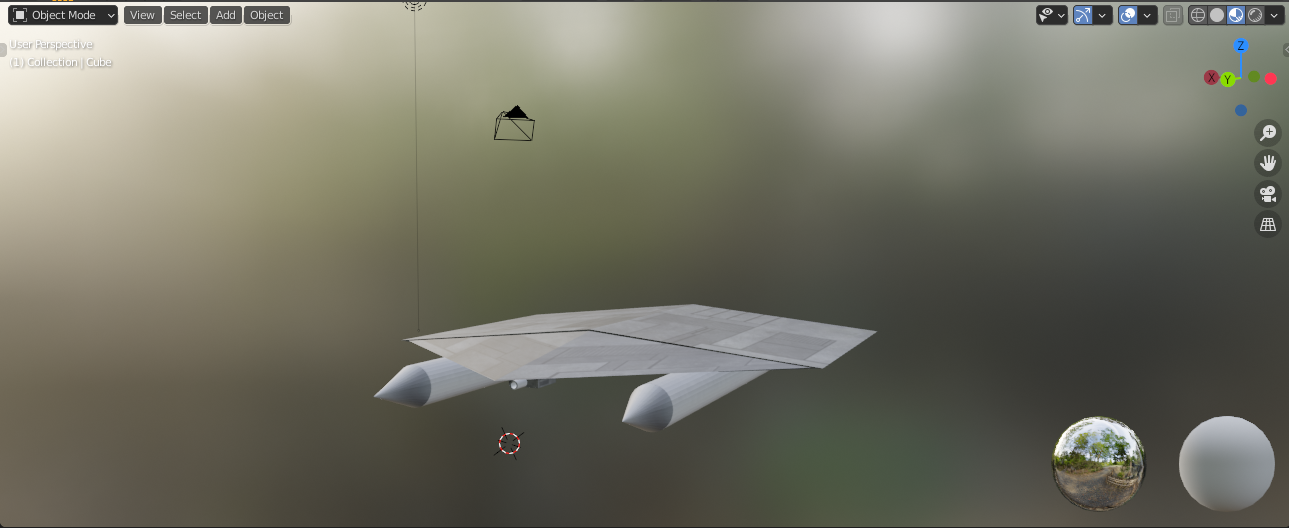
\includegraphics[scale=0.25]{nave.png}
\linebreak
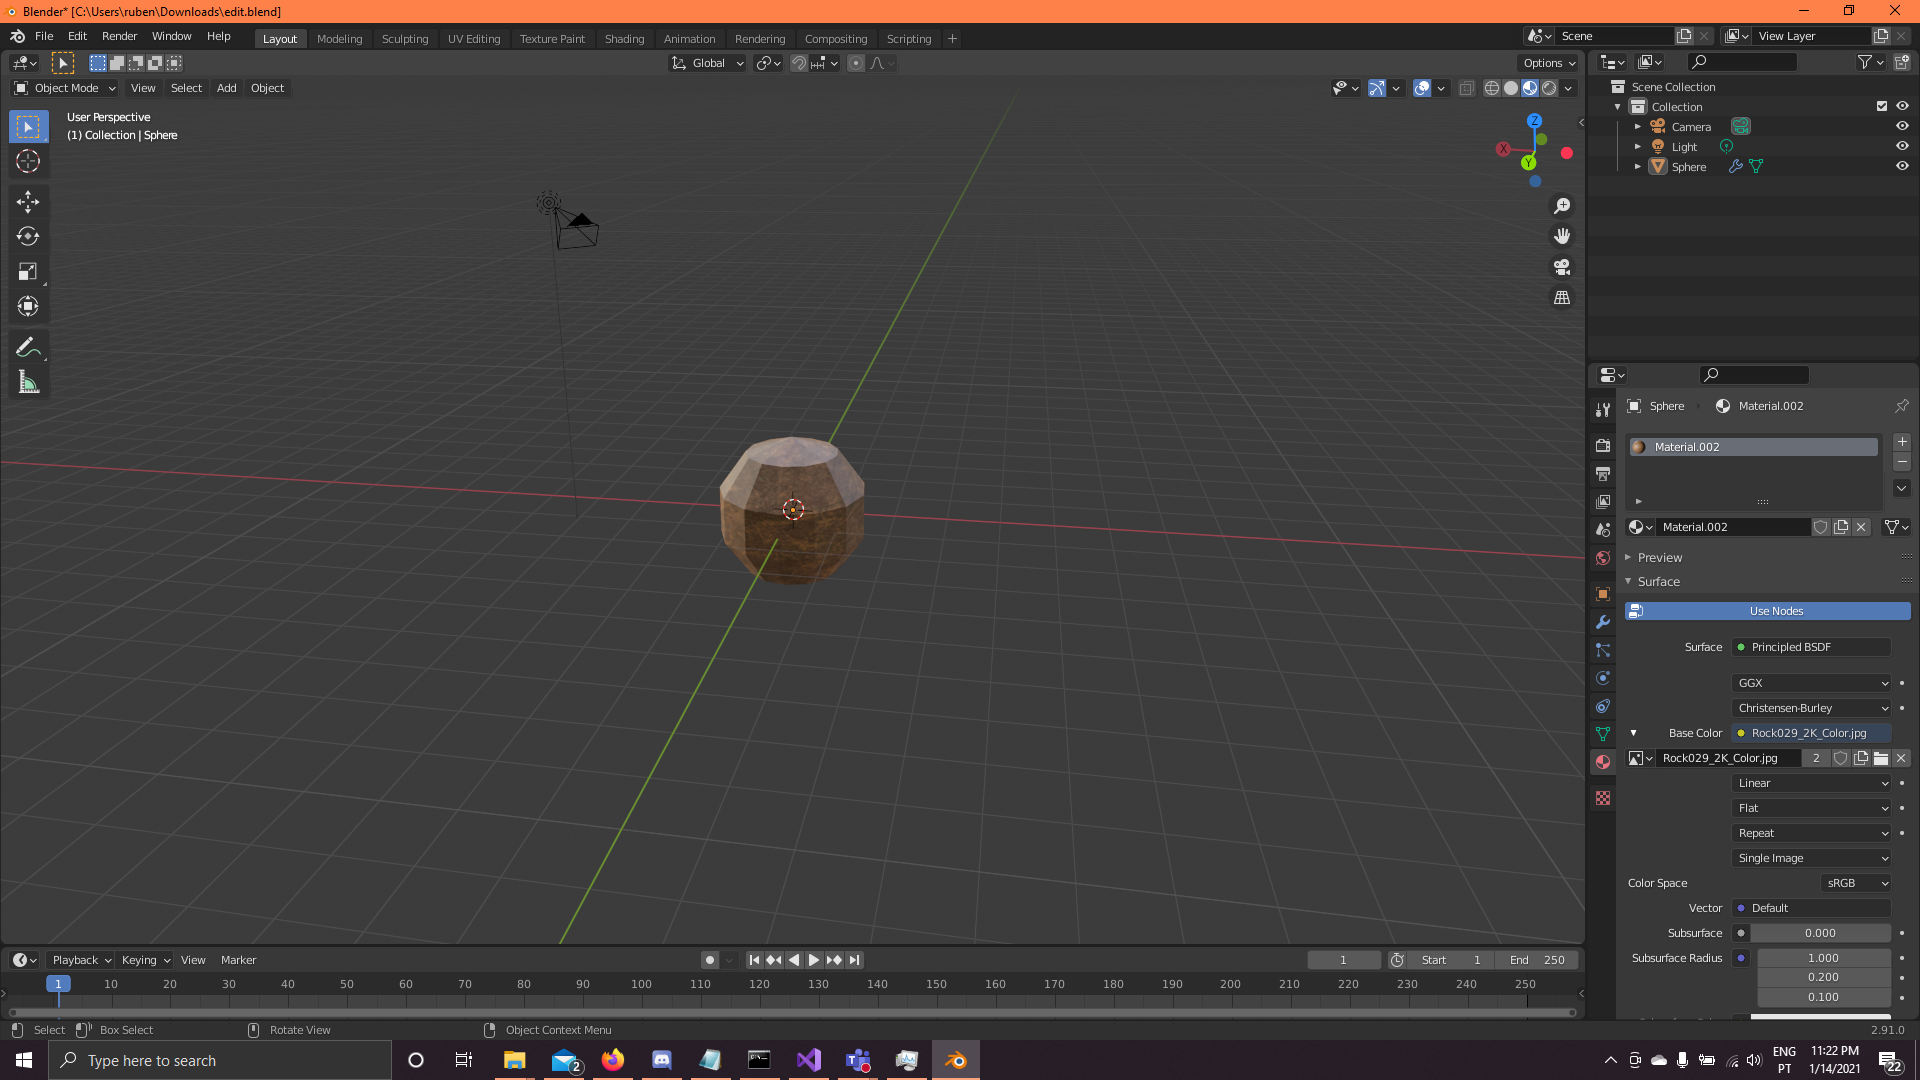
\includegraphics[scale=0.25]{asteroide.png}

\subsection{Interação}
Na fase de desenvolvimento da \textbf{Interação} preocupámo-nos com a escolha de comandos fáceis e intuitivos para manipular a nave. Assim sendo, decidimos utilizar o teclado para a mover, e o rato para controlar a mira da nave e a descarga de plasma para destruir os asteróides.
\subsection{Shaders}
No projeto temos 3 tipos de \textbf{Shaders}, um para as texturas, um para o texto e outro para dar load a objetos 2d (como a mira). Estes shaders são baseados naqueles encontrados no website learnopengl.
\subsection{Texturização}
A \textbf{Texturização} dos nossos objetos foi realizada conjuntamente com a modelação no Blender.

\section{Funcionalidades Extra}
\label{chap4:sec:func-extra}
A equipa de desenvolvimento decidiu implementar algumas funcionalidades extra que achou pertinentes.

\subsection{Texto Gráfico}
Decidimos colocar \textbf{Texto Gráfico} no nosso jogo para melhorar a experiência de utilizador.

\subsection{Sistemas de Pontuação}
Criámos um \textbf{Sistema de Pontuação} para tornar o jogo mais competitivo.

\subsection{2D -> 3D}
Desde a fase de gestão e planeamento do nosso projeto que nunca pensámos em fazer o jogo em 2D dado que queríamos revolucionar o clássico jogo Asteroids com uma versão em 3D.

\subsection{Menus}
Desenvolvemos alguns menus para o nosso jogo, nomeadamente: um menu principal, um menu de pausa e um menu de \emph{Game Over}.
\linebreak
\linebreak
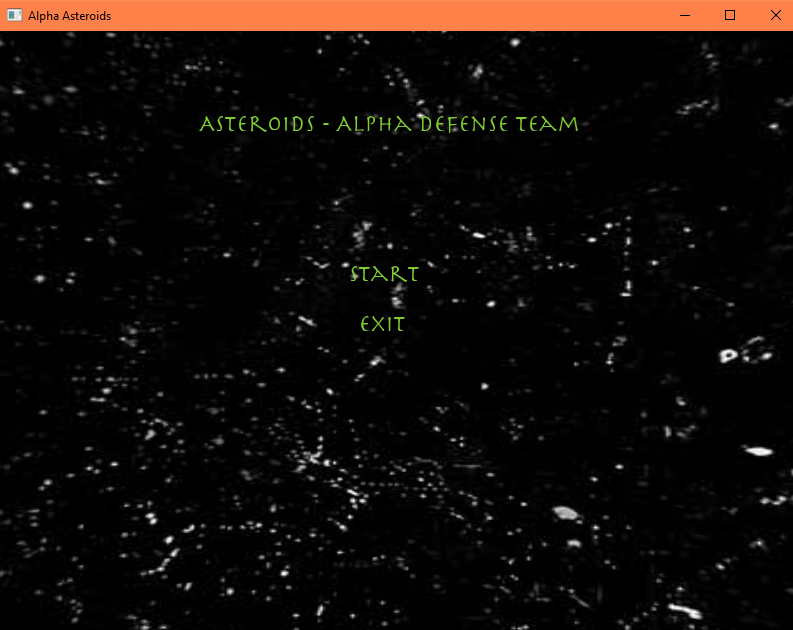
\includegraphics[scale=0.5]{menu.png}